\documentclass[a0paper,dvipsnames, landscape]{tikzposter}

\usepackage[utf8]{inputenc}
\usepackage{adjustbox}
\usepackage{graphicx}

%%%%%%%%%%%%%Bibliography

\usepackage[backend=bibtex,style=verbose-inote,citestyle=authortitle]{biblatex}
\usepackage{xpatch}
\xapptobibmacro{cite}{\setunit{\nametitledelim}\printfield{year}}{}{}
\addbibresource{master.bib}

%%%%%%%%%%%%%%%%%

%%%%%%%%%%%%%%% GRAPHICS


\usepackage{xcolor}
\usepackage{pgfplots}
\usepackage{pgfplotstable}
\usepackage{tikz}
\usetikzlibrary{calc}
\usetikzlibrary{positioning,shapes,arrows, fit, shapes.geometric}

\pgfplotsset{compat=1.8}

\makeatletter
\pgfplotsset{
	/pgfplots/flexible xticklabels from table/.code n args={3}{%
		\pgfplotstableread[#3]{#1}\coordinate@table
		\pgfplotstablegetcolumn{#2}\of{\coordinate@table}\to\pgfplots@xticklabels
		\let\pgfplots@xticklabel=\pgfplots@user@ticklabel@list@x
	}
}
\makeatother


\usepackage{graphicx}


%%%%%%%% Misc

%%%%%%%%%%%%%%%%%%%%%%%%%%%%%%%%%%%


%%%%%%%%% Style
\usetheme{Rays}
\usecolorpalette{GreenGrayViolet}
\usecolorstyle{Spain}


\usepackage[default]{comfortaa}
\usepackage[T1]{fontenc}

\renewcommand\UrlFont{\color{blue}}

\makeatletter

\settitle{ \centering \vbox{
		\tikz[remember picture,overlay]\node[anchor=east,xshift=0.35\linewidth,yshift=-2.5em,inner sep=0pt] {%
					{\includegraphics[scale=0.8]{UWA-Full-Hor-CMYK}}
		};
		\centering
		\color{titlefgcolor} {\bfseries \Huge NovelPersepective \par}
		\vspace*{0.5em}
		{\huge  Identifying Point of View Characters \par}
		\vspace*{1em} {\LARGE {Lyndon White, Roberto Togneri, Wei Liu, Mohammed Bennamoun}}
	}}

%%%%%%
%PARTS

\pgfplotstableread[header=has colnames,
	columns/TestSet/.style={string type},
	]{%
		TestSet	{First Mentioned} {Most Commonly Mentioned}	{ML Classical Feats.}	{ML Word Emb.}
		{A Song of Ice and Fire \\\small George R. R. Martin}	25	97.65625	97.265625	91.40625
		{Six of Crows\\\small  Leigh Bardugo}	42.8571429	93.4065934	94.5054945	79.1208791
		{Wheel of Time\\\small Robert Jordan}	4.3981481	73.6111111	68.0555556	65.9722222
	}{\res}

\newcommand{\resultsblock}{
	\block{Results}{
		\begin{tikzpicture}
		\begin{axis}[ybar,
		xticklabels from table={\res}{TestSet},
		legend style={at={(0.45,-0.35)}, anchor=north,legend columns=2, draw=none},
		legend image post style={xscale=10, yscale=2},
		%	enlargelimits=0.3,
		ymin = 0, ymax=100,
		enlarge x limits=0.3,
		xticklabel style={text width=8em, align=center},
		xtick = data,
		width=0.87\linewidth, height= 15cm,
		bar width=1.9cm,
		yticklabel={$\mathsf{\pgfmathprintnumber{\tick}}$\small\%},
		ytick = {0, 25, 50, 75, 100},
		ylabel = Accuracy,
		xlabel = {\shortstack{Book\\ Series:}},
		x label style={at={(axis description cs:-0.06,-0.01)},anchor=north},
		axis line style={draw=none},
		x tick style={draw=none},
		ytick pos=left,
		nodes near coords={$\mathsf{\pgfmathprintnumber[precision=0]{\pgfplotspointmeta}}$\small\%}
		]
		%\addplot[style={bblue,fill=bblue,mark=none}] table[x expr=\coordindex, y={ML Word Emb.}] {\res};
		\addplot[style={top color=Cyan, bottom color=Blue, draw=none, mark=none}] table[x expr=\coordindex, y={ML Word Emb.}] {\res};
		\addplot[style={top color=Orange, bottom color=Brown, draw=none, mark=none}] table[x expr=\coordindex, y={ML Classical Feats.}] {\res};
		\addplot[style={top color=Gray, bottom color=Purple, draw=none, mark=none}] table[x expr=\coordindex, y={Most Commonly Mentioned}] {\res};
		\addplot[style={top color=Yellow, bottom color=Green, draw=none, mark=none}] table[x expr=\coordindex, y={First Mentioned}] {\res};
		\legend{{\hspace{1cm}Word Embeddings},{\hspace{1cm}Classical Feats.},{\hspace{1cm}Most Commonly Mentioned\hspace{1cm}\null},{\hspace{1cm}First Mentioned}}
		\end{axis}
		\end{tikzpicture}
	}
}

%%
\newcommand{\processblock}{
    	\block{Process}{
    		\resizebox{\linewidth}{!}{
    			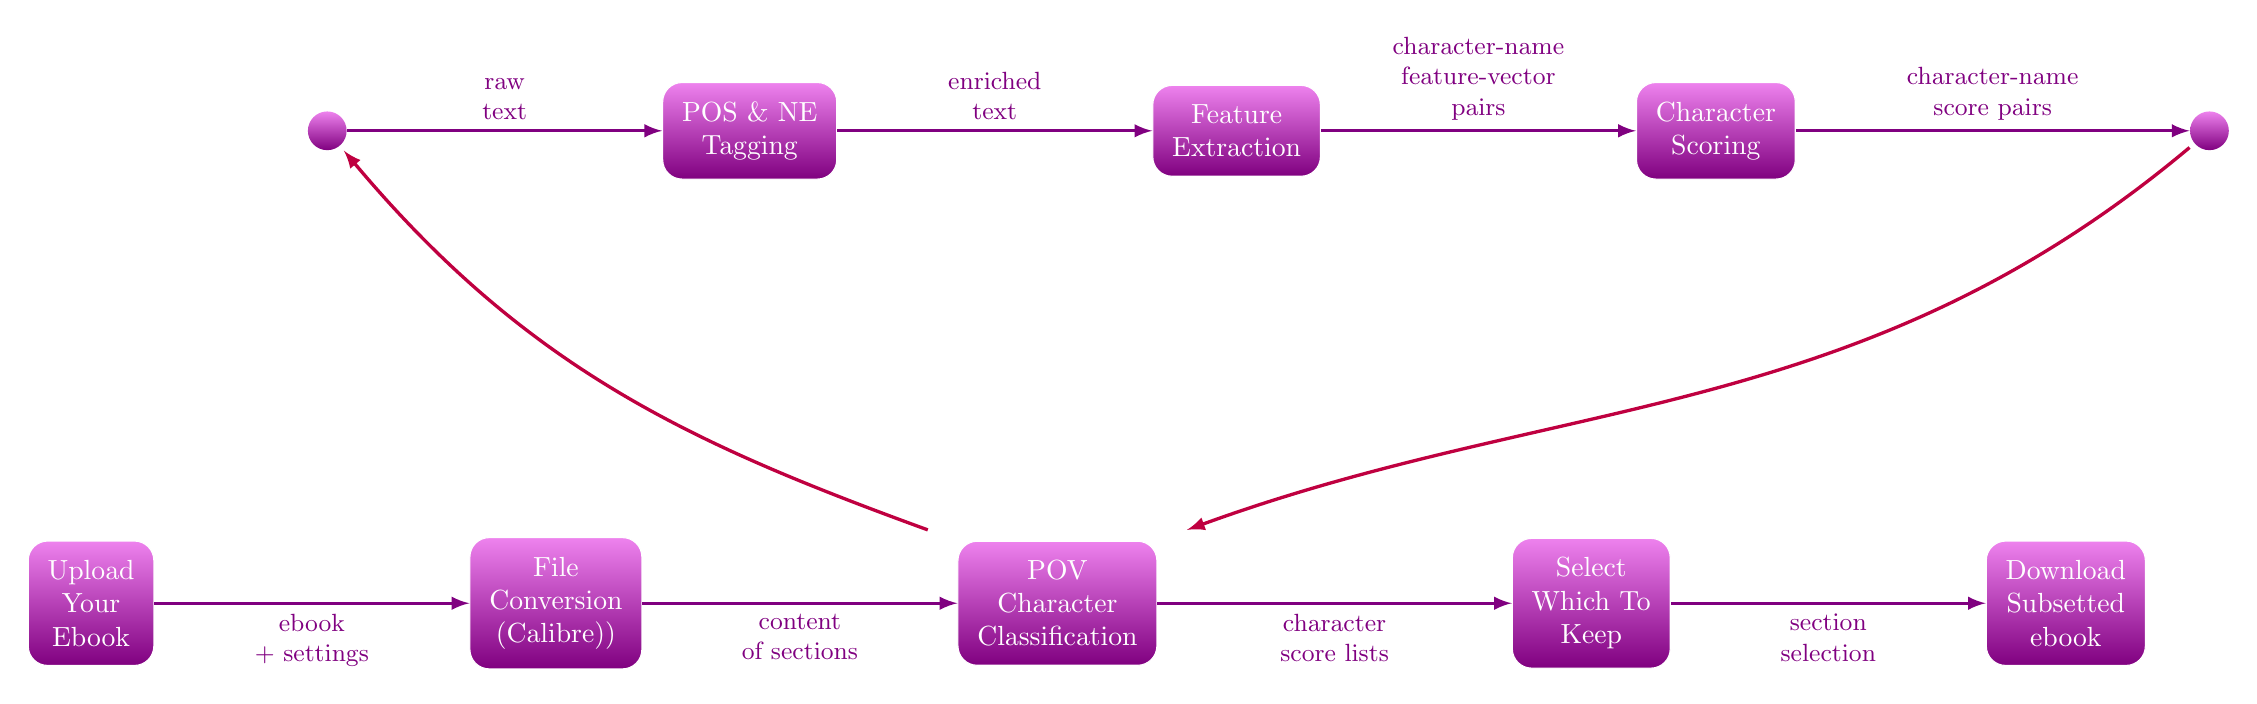
\begin{tikzpicture}[
    			>=latex,
    			every text node part/.append style={align=center},
    			auto,
    			node distance=4, 
    			->,
    			every edge/.append style={very thick, Purple, every node/.style={font=\small}},
    			every node/.append style={rounded corners=7pt, fancy, inner sep=7pt, font=\normalsize},
    			gather/.style = { very thick, purple, shorten <= 0.4cm},
    			fancy/.style= {draw=none, shade, 
    				color=White,
    				top color=Violet, bottom color=Purple
    			}
    			]	
    			\begin{scope}[yshift=6cm]		
    			\node(start1){};
    			\node(enrich)[draw, right=of start1] {POS \& NE \\ Tagging};
    			\node(features)[draw, right=of enrich] {Feature\\ Extraction};
    			\node(scoring)[draw, right=of features] {Character\\Scoring};				
    			\node(end)[right=of scoring, xshift=1cm] {};
    			
    			\path (start1) edge node[]{raw\\ text}  (enrich);
    			\path (enrich) edge node[above]{enriched\\text} (features);
    			\path (features) edge node[above]{character-name\\feature-vector\\pairs
    			} (scoring);
    			\path (scoring) edge node[above]{character-name\\score pairs
    			} (end);
    			\end{scope}
    			
    			\begin{scope}[xshift=-3cm]		
    			\node(start)[draw] {Upload\\ Your \\Ebook};
    			\node(convert)[draw, right=of start, xshift=0.cm] {File\\Conversion\\(Calibre))};
    			\node(classify)[draw, right=of convert, xshift=-0cm] {POV\\Character\\Classification};
    			\node(select)[draw, right= of classify, xshift=0.5cm] {Select\\ Which To \\ Keep};
    			\node(download)[draw, right=of select] {Download \\ Subsetted \\ ebook};
    			
    			\path (start) edge[below] node[below]{ebook \\ + settings}  (convert);
    			\path (convert) edge[below] node[below]{content\\ of sections} (classify);
    			\path (classify) edge[below] node[below]{character\\score lists} (select);
    			\path (select) edge[below] node[below]{section\\selection} (download);	
    			
    			\draw[->, gather] (classify.north west) to[out=160, in=-50] (start1);
    			\draw[<-, gather] (classify.north east) to[out=20, in=-140] (end);
    			\end{scope}
    			\end{tikzpicture}}
    	}
}


%%%%%%%%%%%%%%%%


\begin{document}

\maketitle

\def\gap{\par\vspace{0.5em}}
\begin{columns}
    \column{0.66}
    \begin{subcolumns}
    	\subcolumn{0.5}
	    \block{What? Why? Why are you doing this to books?}{\begin{minipage}{\linewidth}
   	    		Many novels, especially epic fantasy, series a	written from the Point of View (POV) of many different characters. %      
   	    		\gap
   	    		They feature multiple parallel stories tracking the journey of each POV character in parallel.%
   	    		\gap
   	    		As a reader sometimes one wishes to read just one characters story.%
   	    		\gap
   	    		Thus we have made a tool that allows the user to slice-up and restitch their ebooks around a POV character.%
   	    		\gap
   	    		The challenging part is that most books to not label the sections with the name of the POV character, rather the reader works it out.
   	    	\end{minipage}}
   	    	
   	    	
		\block{Source Code}{\centering
			Built on CherryPy, NLTK and Scikit-Learn\\
			https://github.com/oxinabox/NovelPerspective\\
			MIT Licensed\\
		}
    	\subcolumn{0.485}
		\resultsblock{}
    \end{subcolumns}
	
	\def\screenshotwidth{620pt}
	\newcommand{\screenshot}[2]{%
		\innerblock{#1}{\centering\includegraphics[width=570pt]{screenshots/#2}}%
	}
	\block{What does it look like?}{
		\hfill%
		\begin{minipage}[c]{\screenshotwidth}
			\screenshot{Upload your ebook}{startpage}
		\end{minipage}%
		\hfill%
		\begin{minipage}[c]{\screenshotwidth}
			\screenshot{Selection Interface}{controls}
		\end{minipage}%
		\hfill%
		\begin{minipage}[c]{\screenshotwidth}
			\screenshot{Sections are Labelled by POV}{results}
		\end{minipage}
		\hfill
		\null
	}



	\column{0.33} %%%%%%%%%%%%%%%%%%%%%%%%%%%%%%%%%%%%%%%%%%%%%%%%%%%%%%%%%%%%%%%%%%%%%%%%%%%%%%% 
	\processblock{}

	\block{Baseline Methods}{
		\innerblock{First Mentioned}{
			\textbf{Features}: First occurrence of name in text\\
			\textbf{Scoring}: Earliest mentioned scores highest, $S_i=2^{-rank(f_i)}$\\
			\textbf{Result}: Terrible, often other named entities mentioned earlier.
		}
		\gap
		\innerblock{Most Commonly Mentioned}{
			\textbf{Features}: Number of occurrences \\
			\textbf{Scoring}: Most mentioned scores highest, $S_i=\frac{f_i}{\sum_{\forall j} f_j}$\\
			\textbf{Result}: Solid, but fooled by descriptions focusing on others.
		}
	}
	
    
    	
    	
    	\block{Machine Learning Methods}{
    		\innerblock{Classical Features}{
    			\textbf{Features}: Positional, and occurrence features, plus counts of the part of speech on adjacent words. Total $200$ dimensions.\\
    			\textbf{Scoring}: use logistic regression model on if POV or not, $S_i=\frac{P(f_i)}{\sum_{\forall j} P(f_j)}$\\
    			\textbf{Result}: Really strong. Main characters occur near verbs and grammar.
    		}
    		\gap
    		\innerblock{Word Embeddings}{
    			\textbf{Features}: Concatenate the mean of FastText word embeddings for adjacent words
    			Total $600$ dimensions.
    			\\
    			\textbf{Scoring}: use RBF-SVM model on if POV or not, $S_i=\frac{P(f_i)}{\sum_{\forall j} P(f_j)}$\\
    			\textbf{Result}: Really strong, but due to high dimensionality needs sufficient training data.
    		}
    	}
    	
\end{columns}
\block{}{\centering \fontsize{80}{90}\selectfont  http://novelperspective.ucc.asn.au/}


\end{document}
